\begin{figure}[H]
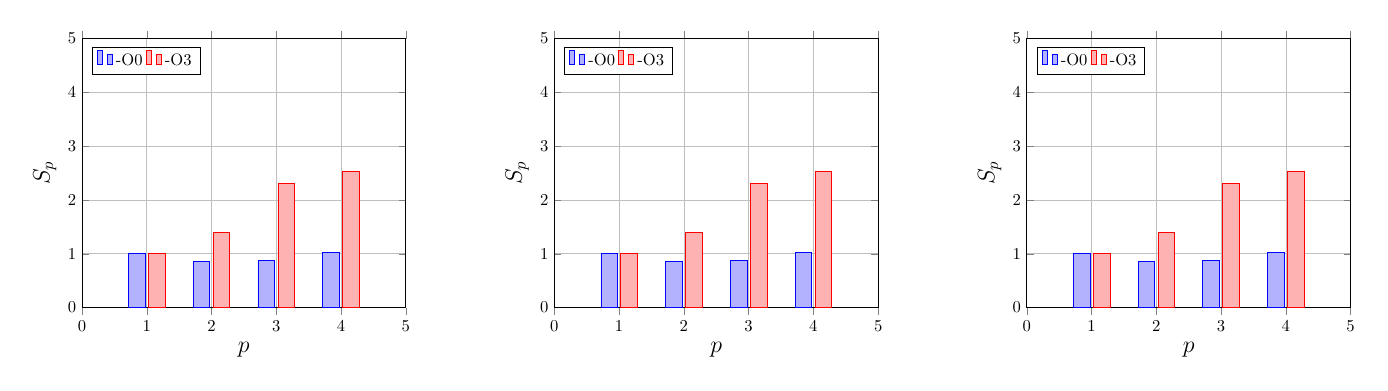
\begin{tikzpicture}
\begin{scope}[scale=0.6]
\begin{axis}[
 ybar,
 xmin=0, ymin=0,
 ymax=5,  xmax=5, %32
 xlabel={\Large $p$}, ylabel={\Large $S_p$},
 grid=major,
legend columns=-1,
legend pos= north west,
tick=empty
]
\addplot coordinates {(1,1) (2, 0.863) (3, 0.869) (4, 1.02)};
\addlegendentry{-O0}
\addplot coordinates {(1,1) (2, 1.4) (3, 2.3) (4, 2.53)};
\addlegendentry{-O3}
\end{axis}
\end{scope}

\begin{scope}[xshift=6cm,scale=0.6]
\begin{axis}[
 ybar,
 xmin=0, ymin=0,
 ymax=5,  xmax=5, %32
 xlabel={\Large $p$}, ylabel={\Large $S_p$},
 grid=major,
legend columns=-1,
legend pos= north west,
tick=empty
]
\addplot coordinates {(1,1) (2, 0.863) (3, 0.869) (4, 1.02)};
\addlegendentry{-O0}
\addplot coordinates {(1,1) (2, 1.4) (3, 2.3) (4, 2.53)};
\addlegendentry{-O3}
\end{axis}
\end{scope}
\begin{scope}[xshift=12cm,scale=0.6]
\begin{axis}[
 ybar,
 xmin=0, ymin=0,
 ymax=5,  xmax=5, %32
 xlabel={\Large $p$}, ylabel={\Large $S_p$},
 grid=major,
legend columns=-1,
legend pos= north west,
tick=empty
]
\addplot coordinates {(1,1) (2, 0.863) (3, 0.869) (4, 1.02)};
\addlegendentry{-O0}
\addplot coordinates {(1,1) (2, 1.4) (3, 2.3) (4, 2.53)};
\addlegendentry{-O3}
\end{axis}
\end{scope}
\end{tikzpicture}
\caption{Ускорение $S_p(p)$ параллельных вычислений, технология OpenMP,\\ 
\mbox{\hspace{2.5cm}}при $N\times N \in \{320\times 320, 640\times 640, 1280\times 1280\}$}
    \label{fig32:Sp}
\end{figure}
